\documentclass[11pt, twoside, openright, a4paper, chapterprefix]{scrbook}
\usepackage[inner=2.5cm, outer=2.5cm, top=4cm, bottom=4cm]{geometry}

%%% PACKAGES %%%%%%%%%%%%%%%%%%%%%%%%%%%%%%%%%%%%%%%%%%%%%%%%%%%%%%%%%%%%%%%%%%
%%%%%%%%%%%%%%%%%%%%%%%%%%%%%%%%%%%%%%%%%%%%%%%%%%%%%%%%%%%%%%%%%%%%%%%%%%%%%%%
%%
%%          $Id: packages.tex 385 2013-02-12 21:53:10Z holz $
%%    author(s): RoboCupAtWork Technical Committee(s)
%%  description: List of packages for the RoboCupAtWork rulebook
%%
%%%%%%%%%%%%%%%%%%%%%%%%%%%%%%%%%%%%%%%%%%%%%%%%%%%%%%%%%%%%%%%%%%%%%%%%%%%%%%%
\usepackage{soul}

\usepackage[english]{babel}
\usepackage{amsmath,amssymb,amsfonts}
\usepackage[nice]{nicefrac}
\usepackage{siunitx}
\usepackage{graphicx}
\usepackage{multicol}
\usepackage{verbatim}
\usepackage{fancyhdr}
% \usepackage{svn-multi}
\usepackage{color}
\usepackage{xcolor,colortbl}
\usepackage{epsfig}
\usepackage{makeidx}
\usepackage{lscape}
\usepackage{pdflscape}
\usepackage{picinpar}
% \usepackage{./styles/bar}
\usepackage{./styles/tweaklist}
%\usepackage{subfigure}
\usepackage{enumerate,paralist}
\usepackage{multirow}
\usepackage{pgffor}
\usepackage{array}
\usepackage{etoolbox}
\usepackage{hyperref}
\usepackage{tabularx}
\usepackage{xspace}
\usepackage[colorinlistoftodos]{todonotes}

%\usepackage[utf8x]{inputenc}
%\usepackage{times}
%\usepackage{helvet}
%\usepackage{courier}

\usepackage{url}
\usepackage{caption}
%\usepackage{subcaption}
\usepackage{epstopdf}
\usepackage{subcaption}
\usepackage{float}
\usepackage{wrapfig}
%\usepackage{titlesec}
\usepackage{xfrac}

\usepackage[normalem]{ulem}  % used for \revadd, \revdel, etc.
\usepackage{xspace}  % used for adding spaces to macros, e.g. \RC, \RCAW, etc.
\usepackage[export]{adjustbox}  % used for valign option on images

\usepackage{pgfplots}
\usepgfplotslibrary{polar}

% Local Variables:
% TeX-master: "../Rulebook"
% End:

\usepackage[titletoc]{appendix}
\usepackage{enumitem}
\usepackage{mathtools}
\usepackage{gensymb}
\usepackage[normalem]{ulem}
\setlist{noitemsep}
\usepackage{hhline}
\usepackage{rotating}
\usepackage{tikz}

\usetikzlibrary{arrows}
\usetikzlibrary{calc}
\usetikzlibrary{fit}
\usetikzlibrary{decorations.pathreplacing}
%%% SubfigureSetup %%%%%%%%%%%%%%%%%%%%%%%%%%%%%%%%%%%%%%%%%%%%%%%%%%%%%%%%%%%%
%\renewcommand{\subfigtopskip}{5pt}        % default is 10pt
%\renewcommand{\subfigbottomskip}{5pt}     % default is 10pt
%\renewcommand{\subfigcapskip}{3pt}        % default is 10pt
%\renewcommand{\subfigcapmargin}{7pt}      % default is 10pt

%%% TweakList-Setup %%%%%%%%%%%%%%%%%%%%%%%%%%%%%%%%%%%%%%%%%%%%%%%%%%%%%%%%%%%
\renewcommand{\itemhook}{%                 % modify itemize-spacing
  \setlength{\topsep}{2pt}%
  \setlength{\partopsep}{1pt}%
  \setlength{\itemsep}{-1pt}%
}
\renewcommand{\enumhook}{%                 % modify enumerate-spacing
  \setlength{\topsep}{2pt}%
  \setlength{\partopsep}{1pt}%
  \setlength{\itemsep}{-1pt}%
}
\renewcommand{\descripthook}{%             % modify description-spacing
  \setlength{\topsep}{2pt}%
  \setlength{\partopsep}{1pt}%
  \setlength{\itemsep}{-1pt}%
}

\setkomafont{title}{\normalfont}
\setkomafont{sectioning}{\normalfont\bfseries}
\addtokomafont{caption}{\small}
\setkomafont{captionlabel}{\small\bfseries}
\setkomafont{descriptionlabel}{\normalfont\bfseries}
\renewcommand*{\chapterformat}{\LARGE{Chapter \thechapter}}

\setcounter{secnumdepth}{3}

\setlength{\parskip}{10pt plus 1pt minus 1pt}
\setlength{\parindent}{0pt}

%%% MACROS %%%%%%%%%%%%%%%%%%%%%%%%%%%%%%%%%%%%%%%%%%%%%%%%%%%%%%%%%%%%%%%%%%%%
\newcommand{\YEAR}{2021\xspace}
\newcommand{\STATE}{Preliminary version}

\input{./setup/macros.tex}
\input{./setup/abbrevix.tex}

\makeindex                                % generate index
\makeabbex                                % generate abbreviations

%%% DOCUMENTINFO %%%%%%%%%%%%%%%%%%%%%%%%%%%%%%%%%%%%%%%%%%%%%%%%%%%%%%%%%%%%%%
\hypersetup{
  pdftitle     = {\RCAW Rulebook},
  pdfsubject   = {\RCAW Rulebook},
  pdfauthor    = {\RCAW Technical Committee},
  pdfkeywords  = {\RC, @Work, Rules, Competition},
  colorlinks   = true,
  anchorcolor  = blue,
  linkcolor    = blue,
  urlcolor     = blue,
}

%%% HEADINGS & PAGE STYLE %%%%%%%%%%%%%%%%%%%%%%%%%%%%%%%%%%%%%%%%%%%%%%%%%%%%%
\newcommand{\footline}{\RCAW Rulebook / \rulebookVersion}
\pagestyle{fancy}
\renewcommand{\chaptermark}[1]{\markboth{\chaptername\ \thechapter. \ #1}{}}
\renewcommand{\sectionmark}[1]{\markright{\thesection \ #1}{}\renewcommand{\currentTest}{#1}}
\fancyhf{}
\fancyhead[LE,RO]{\thepage}
\fancyhead[RE]{\sffamily\rightmark}
\fancyhead[LO]{\sffamily\leftmark}
\fancyfoot[C]{\scriptsize \sffamily \footline{}}
\fancypagestyle{plain}{
        \fancyhf{}
        \fancyhead[LE,RO]{\thepage}
        \fancyhead[RE]{\sffamily\rightmark}
        \fancyhead[LO]{\sffamily\leftmark}
        \fancyfoot[C]{\scriptsize \sffamily \footline{}}
		\renewcommand{\headrulewidth}{0.5 pt}
}
\fancypagestyle{empty}{
        \fancyhf{}
        \fancyhead{}
        \fancyfoot[C]{\scriptsize \sffamily \footline{}}
		\renewcommand{\headrulewidth}{0 pt}
}

\newcommand{\quotes}[1]{``#1''}
\newcommand{\textbi}[1]{\textbf{\textit{#1}}}
%\newcommand{\sectionbreak}{\clearpage}
%\newcommand{\subsectionbreak}{\clearpage}


%%%%%%%%%%%%%%%%%% Please add your personal makro here %%%%%%%%%%%%%%%%%%%%%%%%
\newcommand{\szug}[1]{\todo[color=green!40, inline]{[Sebastian] #1}}
\newcommand{\jon}[1]{\todo[color=blue!40, inline]{[Jon     ] #1}}
\newcommand{\marco}[1]{\todo[color=green!40, inline]{[Marco     ] #1}}
\newcommand{\deebul}[1]{\todo[color=yellow!40, inline]{[Deebul     ] #1}}
\newcommand{\christoph}[1]{\todo[color=teal!40, inline]{[Christoph     ] #1}}
\newcommand{\all}[1]{\todo[color=red!40, inline]{[all     ] #1}}

%%%%%%%%%%%%%%%%%%%\renewcommand{%%%%%%%%%%%%%%%%%%%%%%%%%%%%%%%%%%%%%%%%%%%%%%
%%%%%%%%%%%%%%%%%%%%%%%%%%%%%%%%%%%%%%%%%%%%%%%%%%%%%%%%%%%%%%%%%%%%%%%%%%%%%%%
%%%%%%%%%%%%%%%%%%%%%%%%%%%%%%%%%%%%%%%%%%%%%%%%%%%%%%%%%%%%%%%%%%%%%%%%%%%%%%%

\begin{document}
\errorcontextlines 10000
\listoftodos
% !TEX root = ../Rulebook.tex

\begin{titlepage}
  \begin{center}
    {

      \includegraphics[width=\textwidth]{images/logo_RoboCupAtWork.pdf}\\[1.23ex]
    }
    \vspace{2.7 cm}
    \hrulefill\par
    {%
      \vspace*{.27cm}
      \Huge{\RCAW}\\[1.23ex]
      \Large Rulebook \\[2ex]
    }

    \hrulefill\par

    \vfill
    Asadollah Norouzi\\
  	Sebastian Zug\\
    Deebul Nair \\
    Christoph Steup \\
    Marco Masannek\\
    Maximilian Hachen\\
    Lucas Reinhart
    \vfill
    ~~ Version: \YEAR ~~ \\
    ~~  \today ~~ \\
    %\vfill
  \end{center}

\newpage

\section*{Acknowledgments}

We would like to thank to previous @Work members that supported the league and
advanced the rulebook over years:

Jan Carstensen \\
Frederik Hegger\\
Nico Hochgeschwender \\
Daniel Kaczor \\
Robin Kammel \\
Alexander Moriaty \\
Walter Nowak \\
Benjamin Schnieders\\
Armin Shahsavari \\
Jon Martin \\


In July 2019 our league lost one of the initiators and founding members. Prof. Dr. Gerhard
Kraetzschmar has been very active in many functions within the RoboCup-Community
for decades. We are grateful for his efforts, advises and motivation and will respect his memory.

\section*{How to cite this rulebook}

If you refer to the rulebook in particular, please cite:

\begin{verbatim}
@misc{rulebook_2020,
  author = {Asadollah Norouzi, Sebastian Zug, Deebul Nair,
            Christoph Steup, Marco Masannek, Lucas Reinhart, Maximilian Hachen},
  title  = {RoboCup@Work 2020 - Rulebook},
  year   =  2020,
  howpublished = {\url{https://atwork.robocup.org/rules/}},
}
\end{verbatim}

\end{titlepage}


\pagestyle{empty}

%\listoftodos[Todos, Discussions, Remarks]

\tableofcontents
\clearpage

\pagestyle{plain}

% !TEX root = ../Rulebook.tex

\chapter{Summary of Changes}

This chapter provides an overview for experienced teams that know the rules and just need an update on what is new for the specific year. 
All new teams are strongly advised to read the whole rule book thoroughly.

\section{Adjustments for the virtual RoboCups}

Due to the Covid-19 pandemic, the 2020 and 2021 international robocups are cancelled. 
Some of the leagues, including the RoboCup@Work league, will be held online.
As this brings new challenges for the teams (e.g. arena building) and the committees (comparing teams and scoring),
the technical committee decided to set some rules regarding the arena setup, scoring and the general participation rules.

These can be found in chapter \ref{cha: VRC}.  


\section{General Changes}
\begin{itemize}
  \item BNT will be excluded from the instance list. According to the adapted scoring of the last year (rewards for reaching correct destinations) a separate run focusing on navigation is not necessary anymore.
  \item The preparation time was increased to 3 minutes (1 minute in 2019).
  \item The classification of a collision (major/minor) is more specific now (see \ref{tab:collisions}).
  \item The refbox avoids object distribution patterns, where one manipulation zone is target AND source of
\end{itemize}

\section{Robot Requirements}
\begin{itemize}
  \item The size constraints for the robots were removed to allow more versatile robot designs. 
  		However, the arena specification declares 80 cm as the minimum distance between fixed arena elements.
  		Teams with bigger robots will have disadvantages regarding navigation, as they may get stuck in narrow arena passages. 
  		See \marco{add reference here}.
\end{itemize}

\section{Team Requirements}
\begin{itemize}
  \item
\end{itemize}

\section{Rewards}
\begin{itemize}
  \item
\end{itemize}

\subsection{Technical Challenges}
\begin{itemize}
  \item
\end{itemize}



\chapter{Introduction}
\input{./general_rules/At_Work_in_a_Nutshell}
\section{Organization of the League}\label{sec:organisation_of_the_league}

\subsection{League Committees}
The following list of committees is implemented for \RCAW.

\subsubsection{Executive Committee}

\iaterm{Executive Committee}{EC} members are responsible for the long term goals of the league and thus have also contact to other leagues as well as to the \RC Federation. The EC presents the league and its achievements to the \RC Federation every year and gets feedback to organize the league. All EC members are also members of the Technical Committee. EC members are elected by the Board of Trustees and appointed by the President of the \RC Federation, they serve 3-year terms. The current EC members are:

\begin{itemize}
	\item Asadollah Norouzi, \textit{Singapore Polytechnic}
	\item Sebastian Zug, \textit{University of Mining and Technology Freiberg}
\end{itemize}


\subsubsection{Technical Committee}
The \iaterm{Technical Committee}{TC} is responsible for technical issues of the league, most notably the definition of the rules, such as compliance of the robots with rules and safety standards, the qualification of teams, the adherence to the rules as well as the resolution of any conflicts that may arise during competition. The current TC members are:

\szug{Please check the correctness of members affilation!}

\begin{itemize}
    \item Christoph Steup, \textit{Otto von Guericke University Magdeburg}
    \item Marco Masannek, \textit{Nuremberg Institute of Technology}
	\item Maximilian Hachen, \textit{Leibniz-University Hannover}
	\item Lucas Reinhart, \textit{University of Applied Sciences Würzburg-Schweinfurt}
    \item Nicolas Chia, \textit{???}
		\item Torsten Jandt, \textit{Bonn-Rhein-Sieg University}
    \item Deebul Nair, \textit{Bonn-Rhein-Sieg University}
		\item Pablo Negrete, \textit{???}
    
\end{itemize}


\subsubsection{Organizing Committee}
The \iaterm{Organizing Committee}{OC} is responsible for all aspects concerning the practical implementation of competition, most notably for providing the competition arenas, ensuring their conformity with the rules, and any objects and facilities required to perform the various tests. Further, the Committee is responsible for assigning space to teams in the team area, the organization and scheduling of meetings, the nomination and scheduling of referees, the scheduling and timely execution of tests and stages, recording and publishing competition results, and any other management duties arising before, during, and after a competition. The current OC members are:

\begin{itemize}
    \item Nils Harder, \textit{Otto von Guericke University Magdeburg}
    \item Sjriek Alers, \textit{???}
		\item Franziska Labitzke, \textit{Otto von Guericke University Magdeburg}
		\item Pouya Mansournia, \textit{???}
    \item Abhishek Padalkar, \textit{Bonn-Rhein-Sieg University}
    \item Oliver Uphus, \textit{Leibniz University Hannover}
		\item Kenny Voo, \textit{???}
\end{itemize}


%\subsubsection{Industrial Advisory Board}

%The role of the Industrial Advisory Board is to ensure the industrial relevance of the tests and the overall competition. It allows representatives from industry to voice interesting new problems, which may be included in existing or new test scenarios.
%\par
%Currently, the Industrial Advisory Board has no members yet.

%\subsubsection{ Research Advisory Board}

%The role of the Research Advisory Board is to ensure that the tests and scenarios are innovative and relevant from a research point of view. The members will be recruited from academic institutions and research organizations.
%\par
%Currently, the Research Advisory Board has no members yet.

\subsection{League Infrastructure}
In order to provide a forum for continuous discussions between teams and other stakeholders, the league builds and maintains an infrastructure consisting of a web site, mailing lists, and repositories for documentation, software, and data. The infrastructure is complemented by a minimum infrastructure to be built and maintained by teams, i.e. teams should eventually create their own web page to which the \RCAW League's web pages can be linked.

\subsubsection{Infrastructure Maintained by the League} \label{ssec:LeagueInfrastructure}

\paragraph{Website}
The official website of \RCAW is at
\begin{center}
\url{https://atwork.robocup.org/}.
\end{center}

This web site is the central place for information about the league. It contains general introductory information plus links to all other infrastructure components, such as a league wiki, the mailing lists, important documents such as this rule book, announcements of upcoming events as well as past events and participating teams.

\paragraph{Mailing Lists}
The league maintains several mailing lists:
\begin{description}
	\item[\texttt{rc-work@lists.robocup.org}] This is the general \RCAW mailing list. Anyone can subscribe, but a real name must be provided either as part of the email address or being specified on the mailing list subscription page. The list is moderated in order to avoid abuse by spammers. New members can subscribe to this list here: \url{http://lists.robocup.org/listinfo.cgi/rc-work-robocup.org}.

	\item[\texttt{rc-work-tc@lists.robocup.org}] This is the mailing list for the TC. Posts from non-members have to be approved by the list moderator. Approvals will be given only in well-justified cases.
\end{description}

\paragraph{Repositories}
Several repositories are publicly available under the official \RCAW Github account:
\begin{center}
\url{https://github.com/robocup-at-work}
\end{center}

The repositories provide 3D models for the manipulation objects, their corresponding PPT cavities, and all arena elements. Additionally, the sources to this rulebook, the implementation of the referee box, and various tools can be found.


\subsubsection{Infrastructure Maintained by Teams}
Each team is requested to build and maintain a minimum infrastructure for its team. This infrastructure consist of

\begin{itemize}
	\item team web site,
	\item team contact, and
	\item team mailing address.
\end{itemize}

The team web site should contain the following information:

\begin{itemize}
	\item Name of the team, and team logo, if any
	\item Affiliation of the team
	\item Team leader including full contact information
	\item List of team members
	\item Description of the team's research interest and background
	\item Description of specific approach pursued by the team
	\item Description of the robot(s) used by the team
	\item List of relevant publications by team members

\end{itemize}

The team contact should be the official contact of the team. Usually, for university-based teams, this would be an academic person such as a professor or post-doc, who should, however, be responsive and be able to answer quickly when contacted by email.
\par
The team mailing address should be an email alias, which should be used to subscribe the team to the general \RCAW mailing list. The email alias should at least include the team contact and the team leader.

\section{Participation in the Competition}\label{sec:participation_in_the_competition}
Participation in \RCAW requires successfully passing a qualification procedure. This procedure is to ensure the quality of the competition event and the safety of participants. Depending on constraints imposed by a particular site or the number of teams interested to participate, it may not be possible to admit all interested teams to the competition.
 
\todo[inline]{Needs to be reviewed by Execs}

\subsection{Steps to Participate}
All teams that intend to participate at the competition have to perform the following steps:

\begin{enumerate}
	\item Preregistration (may be optional; currently by sending email to the TC)
	\item Submission of qualification material, including a team description paper, a promotional videos and possibly additional material like designs or drawings
	\item Final registration (qualified teams only)
\end{enumerate}


All dates and concrete procedures will be communicated in due time in advance.

\subsection{Qualification}
The qualification process serves a dual purpose: It should allow the TC to assess the safety of the robots a team intents to bring to a competition, and it should allow to rank teams according to a set of evaluation criteria in order to select the most promising teams for a competition, if not all interested teams can be permitted. The TC will select the qualified teams according to the qualification material provided by the teams. The evaluation criteria will include:

\begin{itemize}

	\item Team description paper
	\item Relevant scientific contribution/publications
	\item Professional quality of robot and software
	\item Novelty of approach
	\item Relevance to industry
	\item Performance in previous competitions
	\item Contribution to \RCAW league, e.g. by
		\begin{itemize}
			\item Organization of events
			\item Provision and sharing of knowledge
		\end{itemize}
	\item Team promo video
	\item Team web site

\end{itemize}

\subsection{Team Description Paper}
The \iaterm{Team Description Paper}{TDP} is a central element of the qualification process and has to be provided by each team as part of the qualification process. All TDPs will be included in the CD proceedings of the \RC Symposium.
The TDP should at least contain the following information in the author/title section of the paper:

\begin{itemize}
	\item Name of the team (title)
	\item Team members (authors), including the team leader
	\item Link to the team web site
	\item Contact information
\end{itemize}


The body of the TDP should contain information on the following:

\begin{itemize}
	\item focus of research/research interest
	\item description of the hardware, including an image of the robot(s)
	\item description of the software, esp. the functional and software architectures
	\item innovative technology (if any)
	\item reusability of the system or parts thereof
	\item applicability and relevance to industrial tasks
\end{itemize}

The team description paper should cover in detail the technical and scientific approach, while the team web site should be designed for a broader audience. Both the web site and the TDP have to be written in English. Alongside the TDP, the TC will - starting 2019 - also require a video file presenting the robot, see Section~\ref{ssec:promotional_video}.

\subsection{Promotional Video}
\label{ssec:promotional_video}
In order to better judge the quality of a team's qualification, the TC asks every team, established or new, to submit a video file describing the robot and its design. The video should clearly demonstrate the robot's ability to perform the tasks required in the challenge, such as autonomous navigation, picking, and placing. Desired elements include visualizing the sensory capabilities of the robot, i.e., seeing what the robot sees, and the plan currently followed by the robot. Spoken language/an audio stream is not required. Ideal video resolution is 1080p with a 16:9 ratio. For large files, please provide a download link.
This file will also be played as explanatory and promotional material during the competiton.

\input{./general_rules/Organization_of_the_Competition}


\chapter{General Rules}
% !TEX root = ../Rulebook.tex

Each of the particular tests defined later in this document may define its own scenario. In this document, a scenario consists of elements such as the

\begin{itemize}
	\item environment,
	\item objects that affect navigation,
	\item objects that are to be manipulated,
	\item objects with which robots interact,
	\item number of robots allowed per team,
	\item number of teams competing simultaneously in the same arena,
	\item task to be performed by a team, and
	\item the criteria for evaluating a team's performance.
\end{itemize}

In order to avoid excessive development efforts for each specific test and to allow reuse of partial functionalities the scenarios are built from a reasonably small set of components, which are later put together in different ways. This section describes these elements.

\section{Design of Robots}
The robots used for competition shall satisfy professional quality standards. The concrete definition of these standards is to be assessed by the TC, comprising aspects such as sturdy construction, general safety, and robust operation. It is not required that the robots are certified for industrial use.

\subsection{Design and Constraints} \label{ssec:RobotDesignAndConstraints}
%The robots need to comply with certain size constraints. A robot, including all parts attached to it as used in the competition, must be able to move by itself into a configuration so that it fits into a box of side lengths 80 cm x 55 cm x 110 cm (length x width x height). If all the robot's parts, such as manipulator or anything able to protrude outside of the previously specified box, are fully extended, the system must still not exceed a box of side lengths 120 cm x 80 cm x 160 cm (length x width x height). The organizers may specify further constraints, such as weight limits. If a team would like to apply a robot with deviating robot dimensions, it should contact the TC. Exceptions for specific robots are possible in case of small differences.

There are no constraints regarding the size and weight of the used robots, but that they have to fit in the arena defined in section \ref{sec:ArenaDesign}. The minimum passage width is 80cm. The used robots must be able to maneuver in that space.\par

The used batteries may not exceed 500Wh of capacity for safety. 300Wh of capacity is recommended. See subsection \ref{ssec:RobotBehaviorAndSafety} as well.\par 

The maximum speed of the robots may not exceed 1.5 m/s. The robot should also be able to halt in a reasonable space on concrete floor.\par 
\par
All robots must have an emergency stop button. The emergency stop has to be a hard stop mechanism, that ensures that the energy transfer to all actuators is stopped immediately and the robot halts. The mechanism must be a red emergency stop button that is clearly visible, easily accessible and per wire attached to the robot. A wireless emergency stop button is optional but not sufficient.
The OC may request the proof of a robot's safety (e.g. the correct operation of an emergency stop) anytime during the competition and exclude teams that cannot satisfy safety requirements.
\par
Electric, pneumatic, and hydraulic actuation mechanisms are permitted, provided that they are constructed and produced according to professional standards and meet safety constraints. Combustion engines and any kind of explosives are strictly forbidden. Robots may not pollute or harm their environment in any way, e.g. by loss of chemicals or oil, spilling liquids, or exhausting gases. Furthermore, constraints on the noise generated by a robot in operation may apply. These will be communicated in due time.
\par
Further, the following assumptions are made about the kind of robots used in the competition:
\par
\begin{itemize}

	\item At least one of the robots used by a team is mobile and moves on wheels. No specific assumptions are made about the kinematic design, but the mobile robots should be able to move on basically flat, sufficiently firm surfaces.
	\item The robots have at least one manipulator and are able to grasp objects, which are graspable by a parallel gripper with a jaw width of at least 5 cm and do not weigh more than 300 g.
	\item The manipulator of the robot should be designed and mounted on the robot such that it can grasp objects from heights between 0 cm and 40 cm above the floor.
	\item The robots use sensors to obtain information about their whereabouts in the environment and the task-relevant objects. The major types of sensors that may be used by the robots include:
	\begin{itemize}
		\item Laser range finders (cf. models by Hokuyo or Sick)
		\item Color CCD cameras (cf. any kind of USB camera)
		\item 3D cameras (cf. any kind of camera with depth information)
	\end{itemize}
	\item The design of the scenario should be such that the robots can solve the tasks safely and robustly using (all or a subset of) these sensors.

\end{itemize}

\par
If there are even vague doubts about the eligibility of using particular designs, parts, or mechanisms, the team should consult the TC well in advance.
\par
The robots have to be marked such that a clear distinction of robots used by different teams during a test is possible for spectators. The OC can define the concrete types of markers to be used. In this case the markers are not taken into account when checking the robot's size constraints. The markers shall not interfere with safe operation of the robot.
\par
The TC may require that robots are equipped with a wireless communication device of some sort (e.g. 802.11n), in order to communicate task specifications to the robots.
\par
Future competitions may foresee the use of RFID sensors in the scenario design.


\subsection{Behavior and Safety} \label{ssec:RobotBehaviorAndSafety}
For safety the robots have to meet the constraints in section \ref{ssec:RobotDesignAndConstraints}. In general, all robots shall be operated with maximum safety in mind. Any robot operation must be such that a robot neither harms humans nor damages the environment. \par 
The used batteries shall be handled with care and all team members must be educated in the correct usage, charging and storage of the batteries of the team. For lithium batteries appropriate storage bags must be used by the teams. The OC supplies a fire extinguisher for lithium batteries at the competition. If this is not sufficient for the used batteries of a team. The team is responsible for supplying an appropriate fire extinguisher by themselfs. The OC and TC control the observance of this rules.

When participating in a competition, the team may operate the robot only in their own team area, in the arenas provided (possibly constrained by a schedule assigning periods of time for exclusive use of the arena by a team or a group of teams), and in any other areas designated by the organizers for robot operation. Any operation of robots outside of these areas, e.g. in public areas or emergency paths, require prior permission by the OC.

\section{Referee Box}
\label{sec:refbox}
The TC shall provide a referee box that supports the evaluation of the competition. It applies the time measuring, generates the tasks according to the chosen test configuration and monitors the
competition. For this purpose each robot has to transmit a keep-alive signal every second during all phases (initialization, preparation, game, finish).

The referee box
\begin{enumerate}
  \item announces the start of the preparation time,
  \item communicates the task specifications,
  \item starts each competition run, and
  \item closes a successful run after reaching the endzone, or
  \item aborts the run in case of a time lapse (indicated by a sound signal of the refbox).
\end{enumerate}

% Figure \ref{fig:refbox} depicts the progress of a competition run.
When the robot is initialized, it starts immediately to transmit its beacon
signal. The referee box answers with a state information. If the previous robot
has left the arena, one of the referees starts the seconded phase by pushing a
button. The referee box transmits a new state message that informs the robot
about the beginning of the initialization phase. Inside the referee box a
timer is started which initiates the start of the execution phase after
transmitting the test parameters. During the run the robot is able to activate
the external devices and to receive their status information. This run phase is
terminated by a second timer that alerts after the duration defined in the
instance table.
%
% \begin{figure}
% \centering
% \input{./tikz/sequence.tikz}
% \caption{Sequence diagram of a complete competition run monitored by the referee box}
% \label{fig:refbox}
% \end{figure}
% \par
The TC provides a \aterm{Robot Operating System}{ROS} based interface of the referee box as well as
a reference implementation.
The Referee box implementation and its documentation is available under the following link:
\begin{center}
\url{https://github.com/robocup-at-work/atwork-commander}

\end{center}



% The publish/subscribe communication with the referee box and the external
% devices have to be mapped on the following topics:\note{We should not talk about @Work being a game, e.g. "gamestate". (Sven and Fred)}

% \begin{table}[h!]
% \centering
%  \begin{tabular}{|l|c|c|p{5.9cm}|}
%  \hline
%  Topic & Robot & Refbox & Remarks \\ \hline\hline
%  {\tt /atwork/refbox/gamestate} & S & P & {\tt uint8 gamestate \newline
% uint8 PREPERATION  = 0\newline
% uint8 RUNNING\_TASK = 1\newline
% uint8 PAUSE    = 2  \newline
% uint8 END\_TASK     = 3\newline
% uint8 STOP     = 4 }\\ \hline
%   {\tt /atwork/refbox/beacon} & P & S & {\tt
%   geometry\_msgs/Pose2D position \newline
% string  current\_action } \\ \hline
%    {\tt /atwork/refbox/taskinfo } & S & P & {\tt BNT[] bnt\_tasks \newline
% BMT[] bmt\_tasks  \newline
% BTT[] btt\_tasks } \\ \hline
%    {\tt /atwork/refbox/[device]/command} & P & S & {\tt int8 state \newline
% int8 ERROR        = -1 \newline
% int8 NOT\_RUNNING  = 0 \newline
% int8 RUNNING      = 1   }\\\hline
%    {\tt /atwork/refbox/[device]/status  } & S & P & {\tt int8 state \newline
% int8 ERROR        = -1 \newline
% int8 NOT\_RUNNING  = 0 \newline
% int8 RUNNING      = 1   }\\\hline
%  \end{tabular}
%   \label{tab:RefBoxTopics}
%  \caption{Referee box topics}
% \end{table}
%
% \begin{table}[h!]
% \centering
%  \begin{tabular}{|l|p{6.3cm}|}
%  \hline
%  Message types & Remarks \\ \hline\hline
%  {\tt Atworkobject} & {\tt uint8 name\newline
% uint8 F20\_20\_B = 0 \newline
% uint8 F20\_20\_G = 1 \newline
% uint8 S40\_40\_B = 2 \newline
% uint8 S40\_40\_G = 3 \newline
% uint8 M20\_100  = 4 \newline
% uint8 M20      = 5 \newline
% uint8 M30      = 6 \newline
% uint8 R20      = 7 \newline
% \revdel{uint8 V20      = 8} \newline
% string destination }\\ \hline
%
%  {\tt BNT} &  {\tt Waypoint[] waypoints }\\ \hline
%
%  {\tt BMT} &  {\tt string   startplace \newline
% string[] pickObjects \newline
% string   destination }\\ \hline
%
%   {\tt BTT} &  {\tt string destination  \newline
% AtworkObject[] objects }\\ \hline
%    {\tt Waypoint  } &  {\tt string position \newline
% uint8  orientation \newline
% uint8  WEST  = 0 \newline
% uint8  EAST  = 1 \newline
% uint8  SOUTH = 2 \newline
% uint8  NORTH = 3 \newline
% uint32  duration  }\\\hline
%  \end{tabular}
%  \caption{Refere box auxiliary message types \todo{can we provide a repository where the message files are stored? And make it consistent with items in Table \ref{tab:manipulation_objects} and \ref{tab:manipulation_objects_rockin}. And add the missing test like PPT, CBT, etc.}}
%   \label{tab:RefBoxAUX}
% \end{table}
%
% Table~\ref{tab:RefBoxAUX} summarizes the auxiliary types embedded in
% the referee box messages. A detailed description of the referee box-API is given in the
% corresponding documentation available on \todo{???????????????}.

\par
The referee box visualizes the current state of the competition run, time measurements, the task specification and robot positions for visitors. Team information (name, affiliation, contact information) are given too in this context.

%\todo{NICO: add maybe some screenshots from the referee box, also make a reference to the FESTO referee box}

\section{Design of the Environment}
\label{sec:ArenaDesign}
\subsection{Size of the Arena}

The size of a competition arena is a rectangular area not less than 2 m x 4 m and not more than 10 m x 12 m. The minimum distance between arena elements(service areas and walls) is 80cm if the passage should be passable for the robot.\par 
An orientation is always associated with the arena. An arbitrary wall is designated as “North” orientation, and the wall to its right is designated as “East” and so on. The orientations will be assigned by the local league chair or/and the TC as soon as the arena is built up. Figure~\ref{fig:example_arena} shows one possible example of an arena configuration, while Figure~\ref{fig:example_topological_map} illustrates the topology.

\begin{figure} [h!]

\includegraphics[width= \textwidth ]{./images/example_arena.jpg}
\caption{An exemplary setup of a \RCAW environment.}
\label{fig:example_arena}
\end{figure}

\begin{figure} [h!]
\includegraphics[width= \textwidth ]{./images/example_map.png}
\caption{Topological map with five service areas (D1, D2, S1, S2, S3). The purple squares define places.}
\label{fig:example_topological_map}
\end{figure}


\subsection{Floor}
The floor is made of some firm material. Examples include floors made of concrete, screed, timber, plywood, chipboard, laminated boards, linoleum, PVC flooring, or carpet. Some examples are illustrated in Figure \ref{fig:example_floors}. Floors may neither be made of loose material of any kind (gravel, sand, or any material which may damage the functioning of the robots' wheels) nor may such material be used on top of the floor. Liquids of any kind are not allowed. The floor may have spots of unevenness of up to 1 cm in any direction (clefts, rifts, ridges, etc.).

\begin{figure} [h!]
\begin{center}
\subfloat[]{\includegraphics[height = 2cm]{./images/example_floor_1.jpg}} \hspace{0.1cm}
\subfloat[]{\includegraphics[height = 2cm]{./images/example_floor_2.jpg}} \hspace{0.1cm}
\subfloat[]{\includegraphics[height = 2cm]{./images/example_floor_3.jpg}} \hspace{0.1cm}
\subfloat[]{\includegraphics[height = 2cm]{./images/example_floor_4.jpg}} \hspace{0.1cm}
\subfloat[]{\includegraphics[height = 2cm]{./images/example_floor_5.jpg}}\\
\subfloat[]{\includegraphics[height = 2cm]{./images/example_floor_6.jpg}} \hspace{0.1cm}
\subfloat[]{\includegraphics[height = 2cm]{./images/example_floor_7.jpg}} \hspace{0.1cm}
\subfloat[]{\includegraphics[height = 2cm]{./images/example_floor_8.jpg}} \hspace{0.1cm}
\subfloat[]{\includegraphics[height = 2cm]{./images/example_floor_9.jpg}} \hspace{0.1cm}
\subfloat[]{\includegraphics[height = 2cm]{./images/example_floor_10.jpg}}
\end{center}
\caption{Examples of floors that can be used for \RCAW arenas.}
\label{fig:example_floors}
\end{figure}

\subsection{Walls and Virtual Walls}

The competition arena is partially surrounded by walls. Parts of the outer border that are not blocked by walls will be
marked by red/white barrier tape and count as virtual walls. The height of the walls is not less than 20 cm and not
more than 40 cm. One or more gates may be foreseen, where robots can enter or leave the arena. Gates are indicated by
blue/wite tape, which may be crossed once per gate without penalty. Most of the walls are supposed to have a uniform
color. Small visual elements like logos or advertisements may be placed on the walls. Virtual Walls are considered
Walls regarding Penalization \ref{sec:ScoringAndRanking}.


\subsection{Barrier Tape} \label{ssec:barrier_tape}

The arena may include virtual fences marked by yellow/black on the floor, which are called Barrier Tapes (see Figure
\ref{fig:barrier_tape}).

The barrier tapes on the floor of the arena mark dangerous zones and are not to be crossed. The penalty for those
collisions can be found under section \ref{sec:penalties}.

The blue/white tape is not considered a barrier tape or a virtual wall but marks the service areas of 0 cm height (see
Section \ref{ssec:serviceareas}).

Blue/White tape is used to frame the entrance and exit area. The robot is allowed to cross this kind of barrier only at
the beginning of a test to enter the arena and at the end for leaving. Consequently, each blue tape not belonging to a
0cm service area may only be crossed once.


\begin{figure} [h!]
\centering
\includegraphics[width= 0.7\textwidth ]{./images/barrier_tapes_in_china15.jpg}
\caption{Example of barrier tape used during \RC 2015. The red/white tape is used to indicate virtual walls , while the yellow/black one denotes a virtual fence.}
\label{fig:barrier_tape}
\end{figure}



\subsection{Entrance and Exit}
If possible, the arena should have one entrance and one exit, which are equipped with laser barriers. These barriers are used for timekeeping by the referee box.


\subsection{Obstacles}

An arena defined for a particular test may foresee the use of obstacles. Obstacles may by passive (i.e. not able to
relocate by themselves) or active (e.g. other robots). The size of obstacles should be not lesser than 10 cm x 10 cm x
5 cm; there is no upper bound on the size, but it is guaranteed that the surface of the obstacle is opaque and not
shiny. The details about the dynamic objects are not known before the competition and will be chosen by the OC or TC
on-site. Examples for obstacles are trash bins, boxes, big aluminium profiles or even other robots.


\subsection{Service Areas} \label{ssec:serviceareas}

Arenas contain one or more service areas, which have specific purposes for a particular test.
Examples include loading and unloading areas, rotating tables, storage areas, etc.
Service areas may contain specific environment objects, such as shelves, racks, etc.
They may be accessible from different locations, i.e. it might be possible to reach an area from two or more sides.
Note that service areas can have different heights, which are fixed at the arena setup time and mantained for the entire cometition.
However, from 2020 on and in order to make the competition more realistic, the heights of the service areas will be variable, allowing the OC to adjust them before each test run.
If a service area has a height of zero cm, a tape will mark the area (see Figure \ref{fig:barrier_tape_0cm}).
The tape will be on the floor and will be blue/white striped.
The surounded area may be covered by a white sheet of paper fixed by the tape.
The OC is responsible to replace it in case of pollution or tears.
This tape may be crossed, and does not count as a collision.
If the robot touches a manipulation object while navigating, this will be handled as a collision.

\begin{figure} [h!]
\begin{center}
\includegraphics[height = 2.5cm]{./images/barrier_tape_0cm_area.jpg}
\end{center}
\caption{Barrier tape used to mark service areas with 0 cm height.}
\label{fig:barrier_tape_0cm}
\end{figure}

Until 2017, service areas have always been represented by white coloured surfaces with no other decoy objects on it than the official ones in Tables \ref{tab:manipulation_objects} and \ref{tab:manipulation_objects_rockin}.
However, this does not represent real life scenarios.
The robot might have to pick objects from different colored or dirty places. Also there could be other industrial items on the surface area that the robot must avoid.
In order to make the operating environment more realistic, different kinds of arbitrary surfaces (Figure \ref{fig:ast_surface_example}) with decoy industrial items (Figure \ref{fig:ast_example}) have been introduced.
To facilitate the participation of newer teams that are yet focused on more basic functionalities, the integration of arbitrary surfaces is by now limited to:
\begin{itemize}
\item One service area during the BTT1.
\item Two service areas during the BTT2.
\item Two service areas during the BTT3.
\item Three service areas during the final round.
\end{itemize}

\begin{figure}[h!]
\centering
\subfloat[]{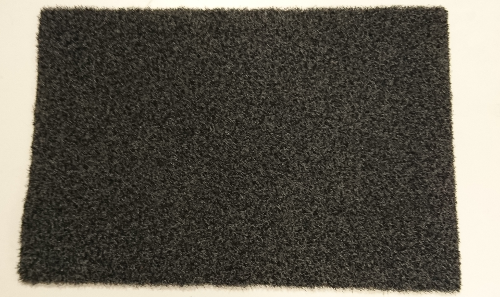
\includegraphics[width=.3\textwidth]{./images/Arbitrary_Surface_rug}}
\hspace{0.5cm}
\subfloat[]{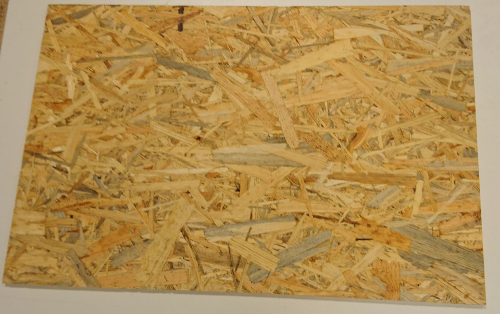
\includegraphics[width=.3\textwidth]{./images/Arbitrary_Surface_wood}}
\hspace{0.5cm}
\subfloat[]{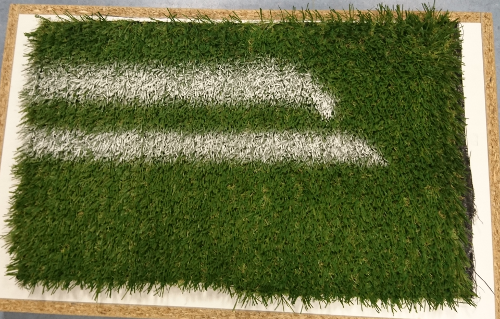
\includegraphics[width=.3\textwidth]{./images/Arbitrary_Surface_grass}}\\
\subfloat[]{\includegraphics[width=.3\textwidth]{./images/Arbitrary_Surface_fake_wood_1}}
\hspace{0.5cm}
\subfloat[]{\includegraphics[width=.3\textwidth]{./images/Arbitrary_Surface_fake_wood_2}}
\caption{Examples of arbitrary surfaces used for service areas.}
\label{fig:ast_surface_example}
\end{figure}

\begin{figure}[h!]
\begin{center}
\subfloat[]{\includegraphics[height = \textwidth/3]{./images/realisticWorkingDeskI.jpeg}}
\hspace{0.5cm}
\subfloat[]{\includegraphics[height = \textwidth/3]{./images/realisticWorkingDeskII.jpeg}}
\end{center}
\caption{Examplary configuration of the working desks}
\label{fig:ast_example}
\end{figure}

\subsection{Containers}
As in many industrial settings, the \RCAW environment may be equipped with several containers (see Figure~\ref{fig:containers}). They can store any kind of manipulation object defined in Section~\ref{ssec:ManipulationObjects}. Robots are supposed either to grasp one or multiple objects out of containers or to place previously grasped objects into them. Several containers can be present in the environment and are always associated with a service area. That means that the container itself will be placed on top and within the manipulation zone defined in Section~\ref{ssec:ManipulationZone}.
It is also possible that more than one container is placed on top of a single service area.
The constraints defined in Section~\ref{ssec:ManipulationZone} apply also to the containers.

Currently, a container itself does to not need to be manipulated or transported by the robot.

\begin{figure} [h!]
\begin{center}
\subfloat[blue]{\includegraphics[height = 3cm]{./images/container_blue.jpg}} \hspace{1cm}
\subfloat[red]{\includegraphics[height = 3cm]{./images/container_red.jpg}}
\end{center}
\caption{Containers can be used for grasping objects out or placing objects into them.}
\label{fig:containers}
\end{figure}

%\subsection{Racks}
%Service areas, e.g. loading and unloading areas, may foresee the use of racks. Objects to be delivered or removed from racks have to be placed or picked up from the top. The height of the racks should be not lesser than 5 cm and not more than 40 cm. The color for the top surface of racks is a bright uniform color such as white or light gray, unless a test specifies a different color. The top surface of the rack may be specially designed in order to serve specific purposes, e.g. holding objects.

\subsection{Shelves}\label{sec:Shelves}
Service areas may foresee the use of shelves and shelf units as depicted in Figure~\ref{fig:shelf}. Objects to be delivered or removed from shelves have to be placed or picked sideways. The height of the shelves should be not lesser than 5 cm and not be more than 40 cm.
The shelf surface may be specially designed in order to serve specific purposes, e.g. holding objects.

\begin{figure} [h!]
\centering
\includegraphics[width=0.4\textwidth ]{./images/shelf.jpg}
\caption{A shelf with two levels and uniform colored surfaces.}
\label{fig:shelf}
\end{figure}

\begin{figure} [h!]
\centering
\includegraphics[width=0.4\textwidth ]{./images/SketchShelf.jpeg}
\caption{Technical draw of shelf configuration.}
\label{fig:shelf}
\end{figure}

\section{Design of Navigation Tasks} \label{sec:NavigationTasks}
Every task has some navigation involved in it. Successful navigation will be awarded in every test according to Table \ref{tab:InstancePoints}. If not defined differently in the respective test, a navigation is successful when the robot reached the service area as defined in section \ref{ssec:Navigating}. 

\textbf{REMARK:} Since 2020 the BNT test is removed from the set of tests done at the competition. Remark that points for reaching service areas are given in all tests, so that teams which are only able to navigate with their robot can still achieve points in all tests.


\subsection{Reaching a Service Area} \label{ssec:Navigating}
A service area counts as successfully reached if the robot would be able to manipulate the service area it is standing on. The manipulation range will be subjectively evaluated by the referees.


\section{Design of Manipulation Tasks} \label{sec:ManipulationTasks}


\subsection{Manipulation Zone} \label{ssec:ManipulationZone}
The manipulation zone defines the area where objects can be placed. Thereby, the following constraints need to be satisfied:
\begin{itemize}
	\item The maximum depth of the manipulation zone is 20 cm.
	\item The minimum distance between objects to each other is 2 cm.
	\item The minimum distance of the beginning of the manipulation zone to a wall is 10 cm.
	\item There as an offset of 2 cm from the border of the service area to the manipulation zone.
\end{itemize}
Note, the constraints do not permit, that objects can be partially occluded dependent on the viewpoint.
\begin{figure} [h!]
\centering
\includegraphics[width=1.0\textwidth ]{./images/manipulation_zone.pdf}
\caption{Manipulation zone: the green color indicates the area where objects can be placed on a service area by the referees.}
\label{fig:manipulation_zone}
\end{figure}


\subsection{Manipulation Objects} \label{ssec:ManipulationObjects}
The manipulation objects in \RCAW shall include a wide range of objects relevant in industrial applications of robotics. They eventually cover any raw material, (semi-)finished parts or products as well as tools and possibly operating materials required for manufacturing processes.
\par
The intention is to start with a simple set of objects of different shapes and colors. Every year, the spectrum shall then be widen in at least one aspect. The initial set of objects includes basic standard screws and nuts with various sizes and masses as shown in Table~\ref{tab:manipulation_objects} and Table~\ref{tab:manipulation_objects_rockin}. Objects of one kind can slightly vary e.g. considering the surface.

For the placement of manipulation objects the following terms are used:

\begin{itemize}
\item Position: point within 2D coordinate system of a service area,
\item Rotation: rotation around vertical axis of a service area,
\item Orientation: rotation around horizontal axes of a service area, i.e. whether the object is standing upright or lying on its side
\item Pose: combination of position, rotation and orientation.
\end{itemize}

\newcommand{\imageView}[1]{\includegraphics[width=2cm, valign=c]{#1}}
{
\newcommand{\rowpadding}{0.4cm}
\setlength\extrarowheight{\rowpadding}
\begin{table}[p]
\begin{tabular}{|c|c|c|m{6cm}|}
\hline
Object & Symbolic Description & Mass & Details \\
\hline
\imageView{./images/F20_20_B.jpg} & \texttt{F20\_20\_B} & 49 g & Small aluminium profile (black)\newline
 Height: 20 mm \newline
 Width: 20 mm \newline
 Length: 100 mm \\ [\rowpadding]
\hline
\imageView{./images/F20_20_G.jpg} & \texttt{F20\_20\_G} & 49 g & Small aluminium profile (gray)\newline
 Height: 20 mm \newline
 Width: 20 mm \newline
 Length: 100 mm \\ [\rowpadding]
\hline
\imageView{./images/S40_40_B.jpg} & \texttt{S40\_40\_B} & 186 g & Big aluminium profile (black)\newline
 Height: 40 mm \newline
 Width: 40 mm \newline
 Length: 100 mm \\ [\rowpadding]
\hline
\imageView{./images/S40_40_G.jpg} & \texttt{S40\_40\_G} & 186 g & Big aluminium profile (gray)\newline
 Height: 40 mm \newline
 Width: 40 mm \newline
 Length: 100 mm \\ [\rowpadding]
\hline
\imageView{./images/M20_100.jpg} & \texttt{M20\_100} & 296 g & Screw\newline
 ISO 4014 \newline
 M20 \newline
 Length: 100 mm \\ [\rowpadding]
\hline
\imageView{./images/M20.jpg} & \texttt{M20} & 56 g & Small nut\newline
 ISO 4032 \newline
 M20 \\ [\rowpadding]
\hline
\imageView{./images/M30.jpg} & \texttt{M30} & 217 g & Big nut\newline
 ISO 4032 \newline
 M30 \\ [\rowpadding]
\hline
\imageView{./images/R20.jpg} & \texttt{R20} & 14 g & Plastic tube\newline
 Inner diameter: 20 mm \newline
 Outer diameter: 30 mm \newline
 Length: 45 mm \\ [\rowpadding]
\hline
%\imageView{./images/V20.jpg} & \texttt{V20} & 14 g & Inner diameter: 20 mm \newline
%Outer diameter: 30 mm \newline
%Length: 45 mm \\
%\hline
\end{tabular}
\caption{\RCAW manipulation object set.}
\label{tab:manipulation_objects}
\end{table}


\begin{table}[p]
\begin{tabular}{|c|c|c|m{6cm}|}
\hline
Object & Symbolic Description & Mass & Details \\
\hline

\imageView{./images/bearingBoxA.jpg} & \texttt{Bearing\_Box} & 102 g & Bearing box\newline
 Height: 25 mm \newline
 Width: 45 mm \newline
 Length: 50 mm \newline
 Inner diameter: 32 mm \\ [\rowpadding]
\hline

\imageView{./images/bearing.jpg} & \texttt{Bearing} & 42 g & Bearing\newline
 Height: 13 mm \newline
 Inner diameter: 15 mm \newline
 Outer diameter: 32 mm \\ [\rowpadding]
\hline

\imageView{./images/axis.jpg} & \texttt{Axis} & 40 g & Axis\newline
 Diameter: 27 mm \newline
 Length: 96 mm \\ [\rowpadding]
\hline

\imageView{./images/distanceTube.jpg} & \texttt{Distance\_Tube} & 5 g & Distance tube\newline
 Height: 10 mm \newline
 Inner diameter: 28 mm \newline
 Outer diameter: 32 mm \\ [\rowpadding]
\hline

\imageView{./images/motor.jpg} & Motor & 20 g & Motor\newline
 Diameter: 42 mm \newline
 Length: 87 mm \\ [\rowpadding]
\hline
\end{tabular}
\caption{RoCKIn manipulation object set.}
\label{tab:manipulation_objects_rockin}
\end{table}
}


\subsection{Grasping Objects} \label{ssec:GraspingObjects}
If not specified differently in a test, the following definition applies to decide if an object counts as being grasped from a service area.
\par
An object counts as grasped from a service area, when the object was moved outside of the source service area. Outside means, that the vertical projection of the object’s convex hull does not touch the service area any more.

\par
The last point shall enable to let the robot pick up an object in order to analyse its type, e.g. by holding it close to a camera on the robot.
\par
If the robot handles an object, but does not fulfill all points above, the object does not count as being grasped, and neither points for grasping a required object, nor penalty points for grasping an unspecified object are given. Still, if the object drops to the ground or an uncontrolled collision occurs, the normal penalty points apply.

\subsection{Placing Objects on Service Areas} \label{ssec:PlacingObjects}
If not specified differently in a test, a manipulation object counts as placed on a target service area if any part of the object is touching the surface of the service area and the object is not moving at the end of the run. An objects does not count as placed when it is dropped (e.g. dropped from a height above 5 cm). This is to avoid that robots throw objects and potentially harm people or property.
\par
The pose of the object on the service area can be chosen freely by the robot.

%\section{Overall Scenario and Variation Points}
%The following two figures illustrate the kind of arenas that can be built with the previously described components. Figure \ref{fig:example_map} shows an old arena configuration (from IROS 2012) as a topological map defining places and connections, while Figure \ref{fig:example_map_go13} shows an arena configuration (from German Open 2013) with only a few surrounding walls, more open space and a conveyor belt.

%\begin{figure}
%\includegraphics[width= \textwidth ]{./images/arena_brsu_spatial_areas.jpg}
%\caption{Illustration of one possible arena configuration. \todo{similar to Figure~\ref{fig:example_arena}. Delete one or put them together in a subfigure environment}}
%\label{fig:example_map_brsu}
%\end{figure}



\chapter{Tests}
% !TEX root = ../Rulebook.tex
\label{sec:tests}

The actual competition contains of a set of so-called tests. 
A test is specified in terms of it's purpose and focus, environment features and eventually manipulation objects involved. Further, a concrete specification of the task is given and the rules to be obeyed. 

Each test has different variability dimensions. That is, which objects to be manipulated, how many locations to visit, from which height to grasp etc. The test instances for \YEAR are defined based on the general test description and can be seen in Section~\ref{sec:ScoringAndRanking}.

\input{./tests/BNT}

\input{./tests/BMT}

\input{./tests/BTT}

\input{./tests/PPT}

\input{./tests/RTT}

%\newpage
%\section{Test Variability} \label{sec:TestVariability}

%The different optional parameters and configurations for each task are 
%mentioned in Section~\ref{sec:ArenaDesign} and \ref{sec:ManipulationTasks}. 
%Figure~\ref{fig:complexityTree} summarizes the possible variations and 
%emphasizes aspects that may be chosen.

%\begin{figure}[ht]
%\centering
%\input{./tikz/complexityTree.tikz}
%\caption{Aspects of variability that may be integrated in a specific instance of a test.}
%\label{fig:complexityTree}
%\end{figure}



\chapter{Scoring and Ranking}
% !TEX root = ../Rulebook.tex
\section{Scoring} \label{sec:ScoringAndRanking}

For each test the calculation of scores is defined individually, comprising points for achieving certain subtasks,
points for winning a run and penalty points.
\par
Each test provides a set of so-called feature variations encoding the overall variability of the test (e.g. whether
obstacles can occur or not, number and type of manipulation objects). To enhance comparability among different test
runs, all teams will have to perform the same test instances as specified in Table~\ref{tab:Instances}.
\par
If not specified otherwise, the following set of scoring rules applies for each test:


Explanation of the terms:
\begin{itemize}
\item Correct navigating is defined in Section \ref{ssec:Navigating}
\item Correct grasping is defined in Section \ref{ssec:GraspingObjects}
\item Correct placing is defined in Section \ref{ssec:PlacingObjects}
\end{itemize}

\section{Simplifications}
Teams may use simplifications, which will result in a reduction of scores for the given run. The simplifications may be
chosen per run, but need to be announced to the referees at least one hour before the start of the run.

\begin{itemize}
	\item Use of external sensors: \hfill -200 points
	\item Use of other external objects (e.g. to support localization): \hfill -100 points
	\item Use of own loading or unloading areas: \hfill -200 points
  \item Deactivation of Barrier Tape: -15\% of total points of the run
\end{itemize}

Additional simplifications are specified for individual tests. These reductions do not count as penalty points. Teams
that want to make use of the simplifications above have to announce them in advance of the competition to the TC. The
TC might forbid the use of specific elements for simplification if these are not in the spirit of the league or may
cause disproportionate advantages for a team.

\section{Penalties}
\label{sec:penalties}
Penalty points are given as follows, each time again the incident occurs:

\begin{itemize}
	\item A manipulation object is dropped to the floor outside of a manipulation area: \hfill -100 points
	\item Delivering a wrong manipulation object to service area \hfill -50 points
	\item Minor collision (see Section \ref{sec:Collisions}): \hfill -50 points
	\item Major collision (see Section \ref{sec:Collisions}): \hfill -50 points and termination of the run
  \item Barrier Tape collision (see Section \ref{sec:Collisions}): \hfill -5\% of total points of current run up till
  20\%
\end{itemize}

\section{Collisions}\label{sec:Collisions}

For reasons of safety of people and property it is strictly unwanted for the robot to collide with any of the
environmental objects. Only collisions of the manipulator with the upside of the service area are allowed. The
different kind of collisions that can occur are defined in the following subsections.

\subsection{Minor Collision}

If the robot collides with an interaction element of the arena (RTT, PPT Cavities, upper level of Shelf) it is
considered a minor collision. The only exception is the collision of the manipulator of the robot with the surface of
the manipulation area.

\subsection{Major Collision}

If the robot collides with a static element of the environment it is considered a major collision.

\subsection{Tape collisions}

\begin{description}
  \item[Yellow/Black Tape]: This tape is called Barrier Tape and represents a virtual fence. If any part of the robot
  touches a barrier tape, it is considered a Barrier Tape Collision. Barrier Tape collision induce a point penalty
  proportional to the final points of the run. With each collision 5\% of the final points are deducted up to a maximum
  of 20\%. For beginner teams the option exists to opt-out of Barrier Tape and take a static deduction of 15\% of the
  final points of the run.
  \item[Red/White Tape]: This tape represents a virtual wall. This wall shall not be crossed. A robot touching this
  tape is considered a major collision. This tape is typically used to limit the area of the arena.
  \item[Blue/White Tape]: This tape is used to indicate 0cm workstations and gates. Robot Collisions with this tape
  only induces a penalty if a gate is crossed twice. In this case a Major Collision occurred.
\end{description}

\begin{table}[h!]
	\caption{Definition of minor and major collisions}
	\label{tab:collisions}
	\centering
  \begin{tabular}{|l|p{1cm}|p{1cm}|p{1.5cm}|}
		\hline
		Situation                                                & Minor & Major & Barrier Tape \\
    \hline
    Collision with static elements of arena                  &       & X     &              \\
    Collision with dynamic elements of arena                 &       & X     &              \\
    Robot Body Collision with workstation                    &       & X     &              \\
    Robot Manipulator Collision with manipulation zone       &       &       &              \\
    Robot Manipulator Collision with Round Table stopping it & X     &       &              \\
    Robot Manipulator Collision with PPT Cavity surface      & X     &       &              \\
    Robot Manipulator Collision with Shelf                   & X     &       &              \\
		Yellow/Black Tape Collisions                             &       &       & X            \\
    Red/White Tape Collisions                                &       & X     &              \\
    Blue/White Tape Collision (1st time gate)                &       &       &              \\
    Blue/White Tape Collision (2nd time gate)                &       & X     &              \\
    \hline
	\end{tabular}
\end{table}

\section{Restarts}
Teams might use one so-called restart in a run. Restarts have the following aspects:

\begin{itemize}

	\item Per run, at most one restart is allowed for a team, if not specified otherwise in a test.
	\item At any time during a run, the team can call for a restart to the referees.
	\item When the referees acknowledge the call for restart, the team may enter the arena. The time will continue running.
	\item The arena and the robot will be reset exactly to the setup at the beginning of the run (except the timer for the run). Random elements such as obstacles or object positions remain like before.
	\item The points for this run achieved so far are reset to zero.
	\item Scores that are received after a restart are multiplied by a factor of 0.75.
	\item The referees decide when the arena is prepared again for the restart. If the robot is not yet ready, teams can keep trying to get it ready until the time for the run is over.
	\item As soon as the team signals that the robot is ready, the task specification is sent again.
	\item Afterwards the start signal is sent from the referee box.

\end{itemize}


\section{Ranking}
The tests will occur in the instances shown in Table~\ref{tab:Instances}. Ranking of the teams will be based on the sum of the achieved points over all the tests.

A team cannot get less than zero points for one run.
The scores of the tests of the first stage are summed up, and the teams with the highest sums proceed to the next stage.

In case of a tie, the OC will either schedule a deciding run or continue with a higher number of participants.

%\setlength{\tabcolsep}{4.75pt}
\renewcommand{\arraystretch}{1.1}
\newcommand{\R}[2]{
	\begin{turn}{90}
		\begin{minipage}[][1em][c]{#2}
		#1
	  \end{minipage}
	\end{turn}
}

\newcommand{\cir}[1]{\hspace{0.5em}\unitlength1ex\begin{picture}(2.8,2.8)%
\put(0.75,0.75){\circle{2.8}}\put(0.75,0.75){\makebox(0,0){#1}}\end{picture}}
\newcommand{\Y}{\tiny \CIRCLE}
\newcolumntype{P}[1]{>{\centering\arraybackslash}p{#1}}

\definecolor{headlineColor}{rgb}{.7,.7,.7}
\definecolor{sectionColor}{rgb}{.7,.1,.1}

\newcommand{\C}{\cellcolor{sectionColor}}

\begin{landscape}
\begin{table}[h!]
 \centering
 \begin{tabular}{|l|l|l*{11}{|P{1cm}}|}
   \hhline{~~~--------}
   \multicolumn{3}{l|}{ }                   &  \multicolumn{8}{c|}{Instances}                        \\
   \hhline{~~~--------}
   \multicolumn{3}{l|}{ }                   &\cir{1}&\cir{2}&\cir{3}&\cir{4}&\cir{5}&\cir{6}&\cir{7} \\
   \multicolumn{3}{r|}{ }                   & BMT   & BTT1  & BTT2  &  BTT3 &  PPT  &  RTT  & Final  \\
   \hhline{~~~--------} \hline
   \multirow{5}{0.5cm}{\R{\centering Objects}{3.0cm}}
   & \RCAW \&  RoCKIn            & RefBox   & 5     & 5     & 6     & 6     & 3      & 3     & 10    \\ \hhline{~----------}
   & Decoy                       & RefBox   &       & 3     & 3     & 3     &        & 3     & 5     \\ \hhline{~----------}
	 & Position                    &          & Ref   & Ref   & Ref   & Ref   & Team   & Ref   & Ref   \\ \hhline{~----------}
	 & Rotation                    &          & Team  & Ref   & Ref   & Ref   & Team   & Team  & Ref   \\ \hhline{~----------}
	 & Orientation                 &          & Team  & Team  & Team  & Ref   & Team   & Team  & Ref   \\ \hline
   \multirow{6}{0.5cm}{\R{\centering Service area}{3.5cm}}
   & Estimated Active            & RefBox   & 2     & 3     & 4     & 5     & 2      & 1     & 8     \\ \hline
   & Table height                & RefBox   &       &       & 0 cm  &       &        &       &  0 cm \\
   &                             &          &       &       & 5 cm  &       &        &       &  5 cm \\
   &                             &          & 10 cm & 10 cm & 10 cm & 10 cm &  10 cm & 10 cm & 10 cm \\
   &                             &          &       &       & 15 cm &       &        &       & 15 cm \\ \hhline{~----------}
	 & Arbitrary surface           & RefBox   &       & 1     & 2     & 2     &        &       & 3     \\ \hline
	 \multirow{3}{0.5cm}{\R{\centering Arena }{1.5cm}}
	 & Obstacles (static)          & Referee  &       &       & 2     & 2     &        &       & 2     \\ \hhline{~----------}
	 & Barrier tape                & Referee  &       & 2     &       & 1     &        &       & 2     \\ \hhline{~----------}
   &                             &          &       &       &       &       &        &       &       \\ \hhline{-----------}
   \multirow{3}{0.5cm}{\R{\centering Grasping }{1.64cm}}
   & Shelf unit                  & RefBox   &       &       &       & 2     &        &       & 2     \\ \hhline{~----------}
	 & Rotating turntable          & Referee  &       &       &       &       &        & 3     & 1     \\ \hhline{~----------}
   & Rotating direction          &          &       &       &       &       &        & Team  & Ref   \\ \hline
   \multirow{8}{0.5cm}{\R{\centering Placement}{2.5cm}}
   & Cavity platform with decoys & RefBox   &       &       &       &       & 3      &       & 1     \\ \hhline{~----------}
   & Shelf unit                  & RefBox   &       &       &       & 1     &        &       & 1     \\ \hhline{~----------}
   & Red container               & RefBox   &       &       &       & 2     &        &       & 2     \\ \hhline{~----------}
   & Blue container              & RefBox   &       &       &       & 2     &        &       & 2     \\ \hhline{~----------}
   & Rotating turntable          & RefBox   &       &       & 1     &       &        &       &       \\ \hhline{~----------}
   & Cavities Position           & RefBox   &       &       &       &       & Ref	   &       & Ref   \\ \hhline{~----------}
   & Cavities Rotation	         & RefBox   &       &       &       &       & Ref    &       & Ref   \\ \hhline{~----------}
   & Cavities Orientation	       & RefBox   &       &       &       &       & Team   &       & Team  \\ \hline \hline
   \multicolumn{2}{|l|}{Duration}
                                 & RefBox   & 5min  & 6min  & 10min & 10min & 4min   & 4min  & 13min \\
 		\hline
 \end{tabular}
 \caption{Test specification in the instances of the \RCAW \YEAR competition.}
 \label{tab:Instances}
\end{table}
\end{landscape}

\begin{landscape}
\begin{table}
 \centering
 \begin{tabular}{|p{5.5cm}*{9}{|P{1cm}}|}
   \hhline{~--------}
   \multicolumn{1}{l|}{}                       & \multicolumn{8}{c|}{Instances}                               \\
   \hhline{~--------}
   \multicolumn{1}{l|}{}                       &\cir{1} &\cir{2} &\cir{3} &\cir{4} &\cir{5} &\cir{6} &\cir{7} \\
   \multicolumn{1}{r|}{}                       & BMT    & BTT1   & BTT2   &  BTT3  & PPT    &  RTT   & Final  \\
   \hhline{~--------}
   \hline
	 Correct service area reached                &   25   &   25   &  25    &   25   &  25    &   25   &   25   \\ \hline
   Correct object grasping standard            &  100   &  100   & 100    &  100   &   0    &        &  100   \\
	 \hspace{0.5cm} round table                  &        &        &        &        &        &  300   &  200   \\
	 \hspace{0.5cm} PPT area                     &        &        &        &        &        &        &  200   \\
	 \hspace{0.5cm} arbitrary surface            &        &  150   & 150    &  150   &        &        &  150   \\
	 \hspace{0.5cm} shelf upper level            &        &        &        &  150   &        &        &  150   \\
	 \hspace{0.5cm} shelf lower level            &        &        &        &  300   &        &        &  300   \\ \hline
   Correct object placing standard             &   75   &   75   &   75   &   75   &        &        &   75   \\
	 \hspace{0.5cm} PPT area                     &        &        &        &        &  200   &        &  200   \\
	 \hspace{0.5cm} shelf upper level            &        &        &        &  150   &        &        &  150   \\
	 \hspace{0.5cm} shelf lower level            &        &        &        &  150   &        &        &  150   \\ \hline
   Incorrect object placing                    & -100   & -100   & -100   & -100   & -100   &        & -100   \\
   Incorrect object grasping                   &        & -100   & -100   & -100   &        & -100   & -100   \\
   Completing whole task                       &   75   &  100   &  150   &  250   &   50   &   75   &  300   \\ \hline\hline
   Maximum attainable points\newline (time bonus not included)
	                                             & 1000   & 1100   & 1400   &  2000  &  700   &  1000  &  3200  \\ \hline
 \end{tabular}
 \caption{Scoring in the instances of the \RCAW \YEAR competition.}
  \label{tab:InstancePoints}
\end{table}
\end{landscape}


\chapter{Virtual RoboCup}
\label{cha: VRC}
% !TEX root = ../Rulebook.tex

\section{General} 
\label{sec:General}

Due to the Covid-19 pandemic, the RoboCup 2021 will be held online. 
Therefore, paricipating teams must provide some infrastructure to enable the TC and OC to evaluate their performance.
This is new for everyone and requires extended communication, which is why every team should join the official discord server:

https://discord.gg/z6Yn6UvhxU

Please participate in discussions and ask questions if you have any.


\section{Arena Setup} 
\label{sec:VRCArenaSetup}

\marco{Kenny pls add your rules here}

\marco{Todo, take example images}


\section{Camera Setup} 
\label{sec:CameraSetup}

\marco{Pls add some kind of sentence regarding the used service (zoom / undecided yet / will be announced}

Since the referees are not present at the arena during the Virtual RoboCup, the arena and all activities of the robot must be shown via livestream. For this purpose, cameras must be able to monitor the entire arena for the referees and the cameras should be mounted at least at head height. No blind spots are allowed when streaming the arena so that the referees can see and evaluate every activity of the robot. One or more cameras can be used to stream the arena. Please contact the OC for the maximum number of streams available.
\par
In addition to the cameras for the arena, there must be a person who follows the robot with a mobile camera and shows the robot's activities from close up. This allows the referees to detect even small mistakes. The person is allowed to enter the arena during the run. However, the person is not allowed to interact with the robot.
\par
A camera may also be attached to the robot to better show the robot's activities to the referees and spectators. The camera on the robot is optional.


\section{Task Generation and Scoring} 
\label{sec:VRCTaskGen}

As normally the refbox would be provided by the OC onsite, no actual refbox will be used during the online competition.
The new refbox implementation, which can be found here (https://github.com/robocup-at-work/atwork-commander), 
gives great opportunity to generate individual tasks for every participating team.

To enable the committee to generate fair tasks for every team, teams must provide detailed information about their arena and object inventory \textbf{1 month} prior to the first competition day. A zip-folder containing the following must be sent via our discord server:

\begin{itemize}
\item Atleast two images of the arena from different perspectives. If two cannot cover the whole arena, teams must provide as many as needed.
\item A map of the arena with workstations marked (name + height). Teams may use an RVIZ screenshot containing \textbf{only} the grid (1m cell size) and the occupancy grid (your map), which may be annotated using e.g. gimp.
\item A list of available workstations in their arena (height and amount).
\item Images of the available arbitrary surfaces
\item Images of the available barriertape and obstacles
\item A list of available objects and containers (amount)
\item Image of the objects and containers
\item Images of the robot (all sides)
\item Robot dimensions in meter
\item Which tests the team intends to participate in
\end{itemize}

The folder must be named VRC2021-info-TEAM-NAME and shall contain the subfolders ARENA, OBSTACLES, OBJECT, ROBOT, TESTS. 
File names must contain information about the data (e.g. Arena-Image-1) and must not have default names (e.g. IMG2012).

The TC will decide if the individual arenas qualify for the tests defined in \ref{tab:Instances}. 
The main requirements are already specified in \ref{sec:VRCArenaSetup}, while the table describes individual task requirements more precisely.
 
If an arena does not qualify, the TC must notify the team \textbf{3 weeks} before competition starts, 
briefing the team about shortcomings and possible solutions. 
The team then has \textbf{1 week} to follow the TCs advice and provide a new zip-folder.
If an arena does not qualify for a test, the TC may decide to exclude the associated team from those.
If an arena only partly qualifies (e.g. no barriertape available), penalty points may be given to teams.
Those penalties will resemble 

The OC will create the tasks for the tests using the official refbox and the information provided by the teams. 
A bagfile will be recorded, containing all topics published by the atwork\_commander.
To prevent incompatible bagfiles during the competition, 
the OC will provide test bagfiles \textbf{2 weeks} before official competitions begin.
The working parameter and launchfiles will be saved and used to generate the specific task bagfiles for the competition.
Teams must be able to play a bagfile on an external computer, which is connected to the robot via WiFi.

Before a test begins, the OC will announce obstacle placements, object positions and arbitrary surface application to a team \textbf{10 minutes} prior to their timeslot. The task bagfile will be sent out to the team \textbf{5 minutes}  before their official timeslot. 
Those durations may be modified during the competitions if they show to be unsuitable.

The bagfile then must be played to start a competition. 
The OC may count down before a competition (3, 2, 1, go), after which \textbf{only} the enter button may be pressed to start the bagfile. 
The cameraman/-woman must show that to the audience.
The OC will set a timer according to the test durations in \ref{tab:Instances}. 
The run ends when the timer is up, with an optional margin of five seconds due to the possible network delay.

As arena setups will not be easy to compare, no time bonus will be given after a perfect run. 
The rest of the scoring will be the same as in a normal robocup scenario.


\chapter{Technical Challenges} \label{cha:TechnicalChallenges}
% !TEX root = ../Rulebook.tex

In the medium term, the \RCAW aims to transfer specific aspects of industrial scenarios in the tests and to demonstrate the practical applicability of the solutions. The challenges, which are adapted or redefined annually, serve as a test platform for the further development of the competitions. Each technical challenge is separately awarded. That means, teams can participate in any number of them. Hoewever any challenge will only be awarded if at least two teams competed unless the only competing team provided an outstanding performance.

A challenge increases the level capabilities of a robot in \RCAW related to:

\begin{itemize}
  \item \textbf{Variability of the environmental conditions} ... The setup conditions of a run are designed variably including disturbances. The lighting situations in the arena are changed dynamically, the configuration of the tables (height, format) is adapted or manipulation objects are mixed with unknown decoy objects.
  \item \textbf{Complexity of the scenarios} ... New arena elements are involved in a scenario
  or its dimensions (size, duration) are increased. This includes, for example, multi-robot scenarios, assembly tasks or new interaction stations.
\end{itemize}

For a successful implementation either an existing solution has to be increased in robustness or a new approach for an additional task has to be developed. The challenges here lie in the fields of perception, manipulation, navigation and planning.

\begin{figure}[h!]
  \centering
  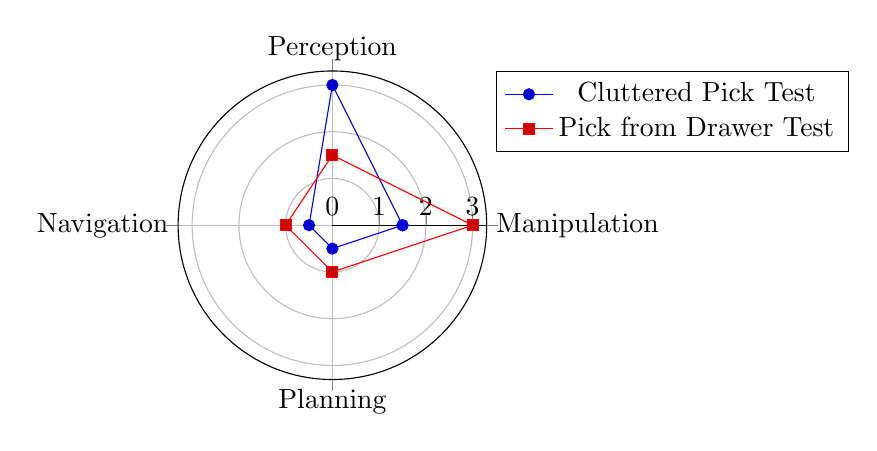
\begin{tikzpicture}
  	\begin{polaraxis}[
        xtick ={0, 90, 180, 270},
        xticklabels= {Manipulation, Perception, Navigation, Planning},
        width=5.5cm,
        height=5.5cm,
        legend pos=outer north east,
    ]
  	\addplot
  		coordinates {(0,1.5) (90,3) (180, 0.5) (270,0.5) (0, 1.5)};  % cp
      \addlegendentry{Cluttered Pick Test}
    \addplot
    	coordinates {(0,3) (90,1.5) (180,1) (270,1) (0,3)};  % pfd
      \addlegendentry{Pick from Drawer Test}
  	\end{polaraxis}
  \end{tikzpicture}
  \label{Examplary Challenge introducing a long term operation based on an extended Final test}
\end{figure}

The challenges of 2021 focussing on perception and manipuation in two scenarios. While "Cluttered Pick Test" (CP) adresses the robustness of perception, the "Pick from Drawer Test" (PFD) is focused on additional complexity by including objects in a drawer. Additonally, the start of a league specific simulator, to ease entry of new teams and enable better scientific evaluation is to be established through Simulation Evaluation Test (SE).


\newpage
\section{Cluttered Pick Test}

\subsection{Purpose and Focus of the Test}

The purpose of the \iaterm{Cluttered Pick Test}{CPT} is to evaluate the perception
and manipulation of the robots when objects are not seperated.

The scenario is motivated by the fact that most of the objects in the factory or 
labs are not perfectly placed but may be stacked or cluttered across a table.

Robots should be able to successfully grasp such objects in a way that they can place them somewhere else.
This ensures that they pick objects regarding potential further use.

\subsection{Scenario Environment}

The scenario is an alternated Basic Manipulation Test, with two service areas with a height of 10cm involved.
All available objects must be placed randomly in a box, which then is emptied above one table. The positions of the objects must remain as they fall. Objects that end up outside of the manipulation zone may be gathered, placed in the box and dropped again. The rule for a minimum distance of 0.02m between objects does not apply for this test. They may be placed near and on top of each other (see \ref{fig:clutter}).

\begin{figure} [h!]
\begin{center}
\subfloat[]{\includegraphics[height = 3cm]{./images/cluttered_pick_1.jpg}} \hspace{1cm}
%\subfloat[]{\includegraphics[height = 3cm]{./images/cluttered_pick_2.jpg}}
\end{center}
\caption{objects places in cluttered environment}
\label{fig:clutter}
\end{figure} 


%\subsection{Variation}
%A slight variation in the competition will be to run with 2 robots simultaneously competing with each other.
%For fairness of the competition the organizers should ensure that the distance between the robot starting
%point and the corresponding service station be equal.

\subsection{Task}

The task is the same as for a BMT, with the modification that only 3 objects must be picked and placed.

\subsection{Rules}
The following rules have to be obeyed:

\begin{itemize}
\item A single robot is used.
\item Three objects have to be picked.
\item There must be atleast 5 decoy objects which must not be picked.
\item The robot has to start from outside the arena and to end in the final.
\item A manipulation object counts as successfully grasped as specified in Section~\ref{ssec:GraspingObjects}.
\item The run is over when the robot reached the final place or the designated time has expired.
\item The order in which the teams have to perform will be determined by a draw.
\item At the beginning of a team's period, the team will get the task specification.
\end{itemize}

\subsection{Scoring}
\begin{itemize}
\item 200 points are awarded for each correctly and successfully picked object
\item 125 points are awarded for each correctly and successfully placed object
\item -100 points for every incorrectly picked object
\end{itemize}

\newpage
\section{Pick from Drawer Test}

%\szug{Should we think about additional rules for collisions?}

\szug{I think an individual drawer avoids unpredictable configurations but generates of course additional effort. Probably we think about a "standard drawer construction" for 2021?}

%\szug{Should we include one or two decoy objects that are placed by a referee to avoid scripted solutions.}

\subsection{Purpose and Focus of the Test}
The collection of freely available objects lying on a manipulation zone is the core capability of \RCAW-robots. The \iaterm{Pick from Drawer Test}{PFD} goes beyond this level and considers objects stored in drawers too. In this way, the challenge
extends the idea of the shelf where the robot has to plan the grasping operation in a limited space but it is not necessary to interact with the environment.

\subsection{Scenario Environment}
The first version of the challenge gives much freedom to the teams. They can choose an arbitrary drawer configuration. The drawer is wholly covered in the beginning and can only be linearly moved in one direction parallel to the floor. The inside of the drawer has to have a uniform color and an uniform flat surface. The surrounding construction has to remain at its position. The inside and the handle of the drawer count as manipulation zones for collision detection purposes.

\par
Robot's movements must open the drawer directly. Self-driven, automatic solutions integrated into the drawer system are not allowed.
The rules do not define the handling mechanism itself, the teams are completely free to design an appropriate concept. Any handle, knob, hole, or connector mounted to the drawer is permitted. Based on this interaction, the drawer has to be moved at least \textcolor{red}{15 cm}. 

\subsection{Task}
The drawer setup is located at an arbitrary position. The drawer contains randoly chosen manipulation objects to be picked described in Table~\ref{tab:Instances}. It is stored directly on bottom of the drawer. Additionally, the drawer may contain three decoy objects and an arbitrary surface. 

The team configures the objects and the drawer during preparation phase.

\textcolor{red}{This test does not adress navigation capabilities. Hence the robot can start the run anywhere in the arena.} It moves directly to the drawer, opens it, grasps the objects and place them in the object inventory of the robot.

\subsection{Rules}
The following rules have to be obeyed:

\begin{itemize}
\item A single robot is used.
\item The test runs for 5 minutes.
\item \textcolor{red}{The robot can start at an arbitrary position inside the arena.}
\item The order in which the teams have to perform will be determined by a draw.
\item Each team is responsible for preparing the drawer system. The team selects the objects and places them within the drawer.
\item The drawer is opened by at least \textcolor{red}{15cm}.
\item A manipulation object counts as successfully grasped as specified in Section~\ref{ssec:GraspingObjects}. \textcolor{red}{It is not necessary to place the objects at another manipulation zone.}
\item The run is over when the designated time has expired.
\end{itemize}

\subsection{Scoring}
\begin{itemize}
\item 100 points for opening the drawer
\item 100 points are awarded for each correctly and successfully picked object, +50 Points per object if decoys are present, +50 Points per object if the Abritrary Surface is present.
\item Time bonus of one point per second after collecting 3 objects successfully.
\end{itemize}

\newpage
\section{Simulation Evaluation Test}

\subsection{Purpose and Focus of the Test}

The purpose of this test is to provide the RoboCup @Work League with new capabilities. These capabilities are the option to do scientific evaluation regarding stochastic behaviour and scalability analysis. This provide the competing teams with the option of using their experimental results in scientific papers and provide a stronger link to the scientific robotic communities.

Another aspect is the option to add integration tests and continuous integration to the workflow of the teams to provide better management of software versions. Additionally, this provides the team members with the capabilities to learn state-of-the-art software development techniques.

Finally, a simulation adds the option for new teams to start with a virtual robot excluding the typical hardware problems associated with real robots. This eases the entry into the league and paves the way for a larger growth of the league in regard to participating teams in the future. 

\subsection{Scenario Environment}

The scenario for this test is to enable teams using a (partial) simulation to show these to the league. Finally, the league may be able to choose a default simulation environment to provide support for this environment in the future. 

Consequently, the simulation of the team competing in this challenge needs to fulfill some requirements:

\begin{description}
  \item[Free to be used:] The simulation software needs to be usable by competing teams free of charge. The software does not need to be open source.
  \item[Open-Source API:] The interface of the simulation needs to be open source. Especially, the implementation of the robot specific functions and behaviours, like executing movement commandos and outputting laser scanner data etc.\ needs to be implemented in a way that allows for easy modification of interested teams.
  \item[Official Models:] The simulated arena environment need to contain the 3D-Model of the official repository of the @Work League \url{https://github.com/robocup-at-work/models}. Additionally, the tasks to be executed need to be generated by the official Referee Box, see Section~\ref{sec:refbox}
\end{description}

  Within the simulation environment one of the tasks specified in Section~\ref{sec:tests} needs to be executed.

\subsection{Task}

The task of this challenge is to show the execution of one of the tasks defined in Section~\ref{sec:tests} in the virtual environment. However, this task is not graded regarding the normal scoring scheme. The evaluation of this task is based on the behaviour of the simulation itself. Relevant aspects that are considered in the scoring are the precision and speed of the simulation. To this end, the teams shall provide stochastic data on the precision of multiple runs of their simulation  as well as the speed of the simulation expressed as a real-time-factor (Quotient between time passed in the simulation and time passed in the real world). Additionally, the teams need to indicate the API of their simulation as well as the used simulation software and its license. The task execution may either be shown in a video or live. 

\subsection{Rules}

\begin{itemize}
  \item Virtual representation based on the object and table definitions from \url{https://github.com/robocup-at-work/models}
  \item Virtual representation of the teams robot
  \item Free to use (for robotic teams) simulation software / environment
  \item Execution of a task as specified in Section~\ref{sec:tests}
  \item Start of task by Referee Box see Section~\ref{sec:refbox}
  \item Task execution as video or live
  \item Indication of precision in form of reproduction accuracy (execute multiple times and compare results)
  \item Indication of simulation speed based on real-time factor (Quotient between virtual clock speed and real world time)
\end{itemize}

\subsection{Scoring}

Referees grade task execution and simulation based on the following criteria:
\begin{itemize}
  \item Up to 100 Points for Ease of Use
  \item Up to 100 Points for Visualization
  \item Up to 200 Points for Precision
  \item Up to 200 Points for Speed
  \item Up to 300 Points for Simulation Capabilities
\end{itemize}






%\chapter{Open Source Award}
%\input{./general_rules/Opensource_Award.tex}


%\input{./tests/BWT.tex}

%\input{./tests/AWT.tex}

%\input{./tests/BAT.tex}



\printabx
\printidx

\end{document}
